% !TEX program = xelatex
\documentclass[11pt,a4paper]{article}

\usepackage[UTF8]{ctex}
\usepackage[margin=2.2cm]{geometry}
\usepackage{amsmath, amssymb, amsthm}
\usepackage{listings}
\usepackage{xcolor}
\usepackage{tikz}
\usepackage{booktabs}
\usepackage{multirow}
\usepackage{hyperref}
\usetikzlibrary{positioning, arrows.meta, shapes.geometric, fit, calc, decorations.pathreplacing}

\hypersetup{
  colorlinks=true,
  linkcolor=blue!60!black,
  urlcolor=teal!70!black,
}

\lstdefinelanguage{Rust}{
  morekeywords={fn,let,mut,pub,struct,impl,use,mod,self,Self,Option,Some,None,return,if,else,for,while,loop,match,break,continue,as,where,trait,type,enum,move,ref,const,static,unsafe,extern,crate,super,dyn,async,await,box,in},
  sensitive=true,
  morecomment=[l]{//},
  morecomment=[s]{/*}{*/},
  morestring=[b]",
}

\lstset{
  language=Rust,
  basicstyle=\ttfamily\footnotesize,
  keywordstyle=\color{blue!60!black}\bfseries,
  commentstyle=\color{green!40!black}\itshape,
  stringstyle=\color{red!60!black},
  numbers=left,
  numberstyle=\tiny\color{gray},
  numbersep=8pt,
  frame=single,
  framerule=0.4pt,
  rulecolor=\color{gray!40},
  breaklines=true,
  breakatwhitespace=true,
  showstringspaces=false,
  tabsize=4,
  columns=fullflexible,
  keepspaces=true,
}

\title{\textbf{halfedge\,: SDF 与 Marching Cubes 模块设计文档} \\ \large \texttt{src/sdf.rs}}
\author{halfedge 库}
\date{2026-07-05}

\begin{document}
\maketitle
\tableofcontents

\section{模块定位}

\texttt{sdf.rs} 实现**有符号距离函数（SDF）**与 **Marching Cubes** 等值面提取，
用于从解析的隐式曲面生成三角网格。这是 halfedge 库中唯一支持
\emph{从连续场到离散网格}生成的模块。

核心内容：
- \texttt{Sdf} trait：有符号距离函数接口（\texttt{eval} + 中心差分梯度）
- SDF 图元：球体、立方体、胶囊体、圆环体
- CSG 组合操作：并集、交集、差集、平滑并集、平移
- Marching Cubes（Lorensen \& Cline 1987）：在均匀网格上提取等值面

\subsection{API 总览}

\begin{center}
\renewcommand{\arraystretch}{1.18}
\begin{tabular}{@{}lp{5.2cm}l@{}}
  \toprule
  \textbf{类型/函数} & \textbf{功能} & \textbf{备注} \\
  \midrule
  \texttt{Sdf} & 距离函数 trait & \texttt{eval} + \texttt{gradient} \\
  \texttt{SdfSphere} & 球体图元 & 中心 + 半径 \\
  \texttt{SdfBox} & 轴对齐立方体 & 半尺寸向量 \\
  \texttt{SdfCapsule} & 胶囊体 & 线段 + 半径 \\
  \texttt{SdfTorus} & 圆环体 & 主/次半径 \\
  \texttt{SdfUnion} & CSG 并集 $\min$ & 泛型 \\
  \texttt{SdfIntersection} & CSG 交集 $\max$ & 泛型 \\
  \texttt{SdfDifference} & CSG 差集 & $A \setminus B$ \\
  \texttt{SdfSmoothUnion} & 平滑并集 & 参数 $k$ \\
  \texttt{SdfTranslate} & 刚体平移 & 偏移向量 \\
  \texttt{march\_sdf} & SDF $\to$ 三角网格 & 采样 + MC \\
  \texttt{march\_field} & 标量场 $\to$ 三角网格 & 纯 MC \\
  \texttt{McParams} & 采样参数 & 原点/体素/分辨率 \\
  \bottomrule
\end{tabular}
\end{center}

\section{SDF 图元公式}

有符号距离函数 $f:\mathbb{R}^3\to\mathbb{R}$：负值在物体内，零值在表面，正值在外。

\begin{center}
\renewcommand{\arraystretch}{1.6}
\begin{tabular}{@{}ll@{}}
  \toprule
  \textbf{图元} & \textbf{SDF} \\
  \midrule
  球体 & $f(\mathbf{x})=\|\mathbf{x}-\mathbf{c}\|-r$ \\
  立方体 & $f=\|\max(\mathbf{q},\mathbf{0})\|+\min(\max(q_x,q_y,q_z),0),\;\mathbf{q}=|\mathbf{x}|-\mathbf{b}$ \\
  胶囊体 & $f=\|\mathbf{p}-\text{proj}_{\overline{ab}}(\mathbf{p})\|-r$ \\
  圆环体 & $f=\|(\sqrt{x^2+z^2}-R,\;y)\|-r$ \\
  \bottomrule
\end{tabular}
\end{center}

梯度默认实现为中心差分：
\[
  \nabla f(\mathbf{x}) \approx
  \left[\frac{f(x+\epsilon)-f(x-\epsilon)}{2\epsilon},\;\ldots,\;\ldots\right],
  \quad \epsilon=10^{-6}
\]

\section{CSG 组合操作}

\begin{center}
\renewcommand{\arraystretch}{1.4}
\begin{tabular}{@{}lll@{}}
  \toprule
  \textbf{操作} & \textbf{公式} & \textbf{说明} \\
  \midrule
  并集 & $\min(f_A, f_B)$ & 取两者较近 \\
  交集 & $\max(f_A, f_B)$ & 取两者较远 \\
  差集 & $\max(f_A, -f_B)$ & $A$ 外 $B$ 内 \\
  平滑并集 & 见下式 & Inigo Quilez \\
  平移 & $f_A(\mathbf{x}-\mathbf{t})$ & 刚体移动 \\
  \bottomrule
\end{tabular}
\end{center}

平滑并集（$k$ 为过渡半径）：
\[
  h=\text{clamp}\!\left(\tfrac{1}{2}+\tfrac{f_A-f_B}{2k},\,0,\,1\right),\quad
  f=\text{mix}(f_A,f_B,h)-k\,h(1-h)
\]

\section{Marching Cubes 算法}

\subsection{原理}

Lorensen \& Cline (1987) 的经典算法，在三维标量场 $f$ 中提取等值面
$\{\mathbf{x}:f(\mathbf{x})=c\}$。对每个体素：

\begin{enumerate}
  \item 采样 8 个角点值，与等值面阈值 $c$ 比较；
  \item 每个角点 $<c$ 记 1，否则 0，拼成 8-bit 案例码 $i\in[0,255]$；
  \item 查 \texttt{EDGE\_TABLE} 得哪些边有交点；
  \item 查 \texttt{TRI\_TABLE} 得三角形拓扑；
  \item 对每条交边线性插值求交点坐标。
\end{enumerate}

\subsection{体素角点与边编号}

\begin{center}
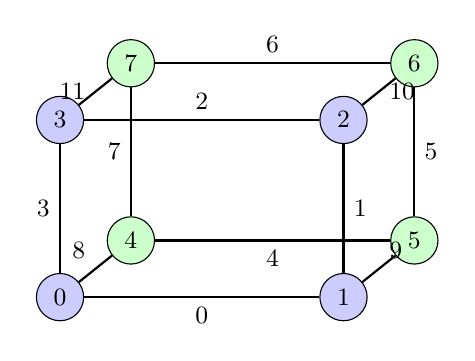
\begin{tikzpicture}[scale=0.9, every node/.style={font=\small}]
  % 底面 0,1,2,3
  \node[draw, circle, fill=blue!20, minimum size=6mm] (v0) at (0,0) {0};
  \node[draw, circle, fill=blue!20, minimum size=6mm] (v1) at (4,0) {1};
  \node[draw, circle, fill=blue!20, minimum size=6mm] (v2) at (4,2.5) {2};
  \node[draw, circle, fill=blue!20, minimum size=6mm] (v3) at (0,2.5) {3};
  % 顶面 4,5,6,7
  \node[draw, circle, fill=green!20, minimum size=6mm] (v4) at (1,0.8) {4};
  \node[draw, circle, fill=green!20, minimum size=6mm] (v5) at (5,0.8) {5};
  \node[draw, circle, fill=green!20, minimum size=6mm] (v6) at (5,3.3) {6};
  \node[draw, circle, fill=green!20, minimum size=6mm] (v7) at (1,3.3) {7};
  % 底面边
  \draw[thick] (v0)-- node[below]{0} (v1);
  \draw[thick] (v1)-- node[right]{1} (v2);
  \draw[thick] (v3)-- node[above]{2} (v2);
  \draw[thick] (v0)-- node[left]{3} (v3);
  % 顶面边
  \draw[thick] (v4)-- node[below]{4} (v5);
  \draw[thick] (v5)-- node[right]{5} (v6);
  \draw[thick] (v7)-- node[above]{6} (v6);
  \draw[thick] (v4)-- node[left]{7} (v7);
  % 竖边
  \draw[thick] (v0)-- node[above left]{8} (v4);
  \draw[thick] (v1)-- node[above right]{9} (v5);
  \draw[thick] (v2)-- node[right]{10} (v6);
  \draw[thick] (v3)-- node[left]{11} (v7);
\end{tikzpicture}
\end{center}

\subsection{边交点插值}

对边 $(a,b)$，设角点值 $v_a, v_b$，等值面 $c$，交点参数：
\[
  t=\frac{c-v_a}{v_b-v_a},\quad
  \mathbf{p}=(1-t)\,\mathbf{p}_a+t\,\mathbf{p}_b
\]
退化（$|v_b-v_a|<10^{-14}$）时取 $t=0.5$。

\subsection{顶点去重}

相邻体素共享边上的交点会被复用。键为 $(i_x,i_y,i_z,e)$（体素索引 + 边编号），
存入 \texttt{HashMap} 去重，避免生成重复顶点。

\section{主算法流程}

\begin{center}
\resizebox{\textwidth}{!}{%
\begin{tikzpicture}[
  node distance=0.45cm,
  proc/.style={draw, rounded corners=2pt, minimum width=11cm, minimum height=0.65cm, align=center, font=\small},
  op/.style={-Stealth, thick},
  startend/.style={draw, rounded corners=10pt, minimum width=3.2cm, minimum height=0.65cm, font=\small, fill=gray!12}
]
  \node[startend] (s) {开始：SDF + 采样参数};
  \node[proc, below=of s, fill=blue!8] (p1) {1. 均匀采样：在 $(n_x\!\times\! n_y\!\times\! n_z)$ 网格上求 $f(\mathbf{x})$};
  \node[proc, below=of p1, fill=blue!8] (p2) {2. 遍历每个体素，8 角点比较阈值得 8-bit 案例码 $i$};
  \node[proc, below=of p2, fill=yellow!15] (p3) {3. 查 \texttt{EDGE\_TABLE[i]} 得交点边集合};
  \node[proc, below=of p3, fill=yellow!15] (p4) {4. 每条交边线性插值求坐标（HashMap 去重）};
  \node[proc, below=of p4, fill=green!12] (p5) {5. 查 \texttt{TRI\_TABLE[i]} 生成三角形};
  \node[startend, below=of p5, fill=green!12] (e) {输出：三角网格 \texttt{MeshStorage}};
  \draw[op] (s) -- (p1);
  \draw[op] (p1) -- (p2);
  \draw[op] (p2) -- (p3);
  \draw[op] (p3) -- (p4);
  \draw[op] (p4) -- (p5);
  \draw[op] (p5) -- (e);
\end{tikzpicture}
}
\end{center}

\section{查找表}

\subsection{EDGE\_TABLE}

\texttt{EDGE\_TABLE[256]} 为 \texttt{u16} 数组，第 $i$ 项的 12-bit 掩码
指示案例 $i$ 中哪些边（0--11）有交点。

\subsection{TRI\_TABLE}

\texttt{TRI\_TABLE[256][16]} 为 \texttt{i16} 二维数组，每行列出案例 $i$
的三角形顶点（边编号 0--11），以 $-1$ 终止。每行最多 5 个三角形
（$5\times 3=15$ 个边编号 + 1 个 $-1$）。

数据来源：Paul Bourke 的经典实现（\url{http://paulbourke.net/geometry/polygonise/}），
通过 \texttt{include!("marching\_table.in")} 在编译期引入。

\section{复杂度}

设分辨率为 $n_x\times n_y\times n_z$（体素数），输出三角形数 $T$，顶点数 $V$。

\begin{center}
\renewcommand{\arraystretch}{1.2}
\begin{tabular}{@{}lll@{}}
  \toprule
  \textbf{阶段} & \textbf{时间复杂度} & \textbf{空间复杂度} \\
  \midrule
  SDF 采样     & $O(n_x n_y n_z)$        & $O(n_x n_y n_z)$ \\
  Marching Cubes & $O(n_x n_y n_z)$      & $O(V+T)$ \\
  顶点去重     & $O(V)$ 平均              & $O(V)$ \\
  \midrule
  \textbf{总计} & $O(n_x n_y n_z)$        & $O(n_x n_y n_z + V + T)$ \\
  \bottomrule
\end{tabular}
\end{center}

\section{退化守卫}

\begin{itemize}
  \item 网格维度 $<2$ 或字段长度不足时返回空网格；
  \item 案例码 $0$ 或 $255$（全内/全外）跳过该体素；
  \item 边端点值差 $<10^{-14}$ 时插值参数取 $0.5$；
  \item 插值参数 $\text{clamp}(t,0,1)$ 防止外推；
  \item 三角形顶点缺失（\texttt{None}）时跳过该三角形而非 panic；
  \item \texttt{add\_triangle} 失败时尝试反向（保证法向一致）；
  \item 胶囊体线段退化（$\|ba\|^2<10^{-14}$）时按点-球处理。
\end{itemize}

\subsection{数据丢弃警告}

当 \texttt{add\_triangle} 创建三角形失败（拓扑冲突）时，\texttt{march\_field}
不再静默丢弃，而是计数并在返回前通过 \texttt{eprintln!} 输出警告：
\begin{center}
\texttt{[halfedge::march\_field] 警告：N 个三角形创建失败（拓扑冲突），已跳过}
\end{center}

\section{测试覆盖}

\begin{center}
\renewcommand{\arraystretch}{1.18}
\begin{tabular}{@{}ll@{}}
  \toprule
  \textbf{测试名} & \textbf{验证点} \\
  \midrule
  \texttt{sdf\_sphere\_center} & 球体中心值为 $-r$，外部为正 \\
  \texttt{sdf\_box} & 立方体内部为负，外部为正 \\
  \texttt{sdf\_torus} & 圆环体环心处值为 $-r_{\text{minor}}$ \\
  \texttt{sdf\_union} & 两球并集中点为负 \\
  \texttt{march\_cubes\_sphere} & 球体 MC 生成顶点/面数 $>0$ \\
  \texttt{march\_cubes\_torus} & 圆环体 MC 生成顶点/面数 $>0$ \\
  \texttt{march\_cubes\_empty} & 全外部场生成空网格 \\
  \texttt{sdf\_gradient} & 球体梯度方向指向外 \\
  \texttt{sdf\_smooth\_union} & 平滑并集在过渡区为负 \\
  \bottomrule
\end{tabular}
\end{center}

全模块共 9 个单元测试；项目整体 \texttt{cargo test} 共 477 个用例。

\section{设计权衡}

\begin{itemize}
  \item \textbf{查找表 vs 算术生成}：
        Marching Cubes 的 256 种案例无法简单算术生成，
        使用预计算查找表（\texttt{EDGE\_TABLE} + \texttt{TRI\_TABLE}）
        是工业标准做法，$O(1)$ 查表，可读且高效。

  \item \textbf{经典表 vs Marching Tetrahedra}：
        经典 MC 在某些案例存在拓扑二义性（面/内部二义性），
        可能产生空洞。本模块采用经典 Lorensen 表（Paul Bourke 版本），
        对大多数应用足够；若需无空洞可改用 Marching Tetrahedra
        （每体素拆 6 个四面体），但三角形数翻倍。

  \item \textbf{泛型 CSG vs trait 对象}：
        CSG 操作用泛型 \texttt{SdfUnion<A,B>} 编译期单态化，
        零开销；\texttt{march\_sdf} 用 \texttt{\&dyn Sdf} 动态分发，
        因为调用方常传入组合后的 SDF 树。

  \item \textbf{顶点去重策略}：
        用 \texttt{HashMap<(ix,iy,iz,e), VertexId>} 去重，
        键为体素索引 + 边编号。相邻体素共享边时复用顶点，
        避免生成重复顶点。代价是 $O(V)$ 哈希表内存。

  \item \textbf{include! 宏 vs 内联常量}：
        \texttt{TRI\_TABLE} 通过 \texttt{include!("marching\_table.in")}
        引入，将 256 行查找表与逻辑分离，便于维护和对照验证。
\end{itemize}

\end{document}
